\documentclass[12pt,a4paper]{article}
\usepackage[utf8]{inputenc}
\usepackage[magyar]{babel}
\usepackage{amsmath}
\usepackage{graphicx}
\usepackage{multirow}

\usepackage{caption}
\usepackage[letterspace=300]{microtype}

\usepackage{atbegshi}
\usepackage{tikz}
\usepackage[left=2cm, right=2cm, top=5cm, bottom=1cm]{geometry}

\title{Igazolás önkéntes tevékenységről\vspace{-1.0cm}}
\date{}
\author{}
\pagenumbering{gobble}

\usepackage{parskip}
\setlength{\parindent}{0pt}

\newcommand\Header{
	\begin{tikzpicture}[remember picture,overlay]
	\fill[blue!40] (-\paperwidth,0.3) rectangle (2\paperwidth, -0.3);
	\fill[white] (\paperwidth/2 - 70,0) ellipse (3.2 and 1.25);
	\node[inner sep=0pt] (picture) at (\paperwidth/2 - 70,0.2){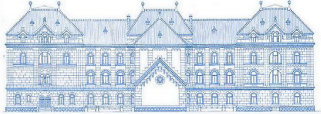
\includegraphics[width=5cm]{epulet.png}};
	\node[inner sep=0pt, text=white] (from) at (2.9, -0.05){\textbf{1 9 1 0  /  1 9 1 1}};
	\node[inner sep=0pt, text=white] (from) at (13.2, -0.05){\textbf{2 0 1 0  /  2 0 1 1}};
	\node[inner sep=0pt, text=blue!75!black] (from) at (\paperwidth/2 - 75,-1.5){\LARGE\lsstyle LUSTRUM SAECULARE COLLEGII};
	\node[inner sep=0pt] (from) at (\paperwidth/2 - 70,-2.5){\large \textit{Szabadon szolgál a szellem}};
	\end{tikzpicture}
}

\newcommand\Footer{
	{\footnotesize 
	\begin{minipage}[t]{0.4\textwidth}
		\begin{flushright}
			ELTE EÖTVÖS JÓZSEF\\
			COLLEGIUM\\
			Dr. Horváth László\\
			igazgató\\
			Kocsis Ábel\\
			választmányi elnök
		\end{flushright}
	\end{minipage}
	\hspace{1em}
	\begin{minipage}[t]{0.45\textwidth}
		\begin{flushleft}
			H-1118 Budapest, Ménesi út 11-13\\
			Tel.: +36 1 460 4481 • Fax.: +36 1 209 2044\\
			E-mail:	titkarsag@eotvos.elte.hu • horvathl@eotvos.elte.hu
			ejc.valasztmany@gmail.com • elnok@eotvos.elte.hu\\
			Honlap: http://www.honlap.eotvos.elte.hu/
		\end{flushleft}
	\end{minipage}
	}
}


\pagestyle{empty}
\AtBeginShipoutFirst{\Header}

\newcommand{\signiture}[3]{
\begin{center}
	#1\\
	#2\\
	#3
\end{center}
}

\begin{document}
\maketitle

Ezúton hivatalosan igazoljuk, hogy <NAME> (Neptun-kód: <NEPTUN>) az ELTE Eötvös József Collegium Választmány munkáját segítve a <SEMESTER>-es félévétől a Választmány belügyi alelnökeként aktívan részt vesz a collegiumi programok szervezésében.\\
\leavevmode\smallskip
Alelnökként
\begin{itemize}
	\itemsep0em 
	\item elősegíti a Collegium gördülékeny belső működését;
	\item felügyeli a Választmány bizottságainak munkáját;
	\item rendszeresen munkakapcsolatot tart fent a gondnoksággal;
	\item felügyeli a Collegium programjainak szervezését;
	\item a választmányi elnök akadályoztatása esetén ellátja annak feladatkörét.
\end{itemize}


\leavevmode\\
Budapest, \today
\vspace{5em}

\begin{flushright}
	\begin{minipage}[t]{0.4\textwidth}
		\signiture{Kocsis Ábel}{elnök}{Eötvös József Collegium Választmány}
	\end{minipage}
\end{flushright}

\vspace{5em}

\begin{flushright}
\begin{minipage}[t]{0.4\textwidth}
	\signiture{Dr. Horváth László}{igazgató}{Eötvös József Collegium}
\end{minipage}
\end{flushright}

\vfill

\begin{center}
	\Footer
\end{center}

\end{document}